\section{External Interface Requirements}
\subsection{User Interfaces}
There are no user interface requirements.

\subsection{Hardware Interfaces}
There are no hardware interface requirements.

\subsection{Software Interfaces}
The \ac{CKB} system relies on the use of the GitHub system in order to manage the battle's repositories. With every new battle created a new repository is generated on Github. Every group of student will then fork this repository and setup a workflow in order to notify the \ac{CKB} system of every new commit through Github.

\subsection{Communication Interfacess}
There are no communication interface requirements.

\newpage
\section{Functional Requirements}
\subsection{Requirements}
The \ac{CKB} system offers several functionalities. In the following table we describe all the requirements that the system should respect in order to achieve its goals.
\begin{center}
    \begin{longtable}{ |l|p{0.85\linewidth}| }
        \hline
            \textbf{ID} & \textbf{Description}\\
        \hline
            R1 & The platform allows a signed in educator to create tournaments \\
        \hline
            R2 & Educators can create battles in the context of a specific tournament they are involved in (Either by creation or by invitation)  \\
        \hline
            R2.1 & The platform allows an educator that created a tournament, to invite other educator and to grant them permission to create battles in the tournament context \\
        \hline
            R2.2 & The platform allows an educator to upload the codekata (description and software project, including test cases and build automation scripts) when creating a battle \\
        \hline
            R2.3 & The platform allows an educator to set subscribtion and submission deadlines when creating a battle \\
        \hline
            R2.4 & The platform allows an educator to set minimum and maximum group size when creating a battle \\
        \hline
            R2.5 & The platform allows an educator creating a battle to include a manual evaluation stage \\
        \hline
            R3 & The platform allows students to subscribe to a tournament \\
        \hline
            R4 & The platform allows a student subscribed to a tournament to join a battle in that tournament context \\
        \hline
            R4.1 & The platform allows students to create a group by inviting other students when joinin a battle \\
        \hline
            R5 & The platform allows Students to login \\
        \hline
            R6 & The platform allows Educators to login  \\
        \hline
            R7 & If manual evaluation is required during consolidation stage the platform allows an educator to go through sources and add a score to the group score \\
        \hline
            R8 & The platform allows all users to view student ranks from previous and current tournaments \\
        \hline
            R8.1 & For every tournament the platform maintains a ranking for students based on the sum of their battle scores \\
        \hline
            R9 & The platform pulls group sources from Github when it receives a notification within the submission deadline \\
        \hline
            R9.1 & The platform analyzes, runs testcases and scores the source of a group solution for a codekata battle and updates the group score accordingly \\
        \hline
            R10 & The platform allows all user to sign in \\
        \hline
            R11 & The platform allows educators to close tournaments  \\
        \hline
            R12 & When a battle deadline expires the platform sets the battle status to consolidation stage  \\
        \hline
            R13 & The platform allows all users who are involved in a battle to look at group ranks for that battle  \\
        \hline
            R13.1 & For every battle the platform maintains a ranking of the groups based on their battle score  \\
        \hline
            R14 & The platform will notify signed students of a newly created tournament  \\
        \hline
            R15 & The platform shall notify students who are subscribed into a tournament that a new battle is available in that tournament context  \\
        \hline
            R16 & The plaftorm shall notify students who are participating in a battle that the final rank for that battle is available  \\
        \hline
            R17 & The plaftorm shall notify students who are subscribed in a tournament that the final rank for that tournament is available  \\
        \hline
            R18 & The platform shall create a new repository with Github for every new battle in any tournament after the submission deadline expires\\
        \hline
            R19 & The platform shall send the battle repository link to students who joined that battle after the submission deadline expires\\
        \hline
    \end{longtable}
\end{center}
\subsection{Mapping on goals}

\begin{center}
    \begin{longtable}{|l|l|p{0.50\linewidth}|}
        \hline
            \textbf{Goal} & \textbf{Domain Assumption} & \textbf{Requirements} \\
        \hline
            G1 & A5, A6 & R1, R11, R6, R10\\
        \hline
            G2 & & R2, R2.1, R2.2, R2.3, R2.4, R2.5, R6, R10\\
        \hline
            G3 & & R3, R14, R5, R6, R10 \\
        \hline
            G4 & A1, A4 & R4, R4.1, R15, R5, R6, R10, R18, R19\\
        \hline
            G5 & A2, A3 & R7, R9, R9.1, R12, R5, R10\\
        \hline
            G6 & & R8, R8.1, R13, R13.1, R16, R17, R5, R6, R10\\
        \hline
    \end{longtable}
\end{center}

\subsubsection{An educator can manage a tournament}

\begin{itemize}
    \item R1: The platform allows a signed in educator to create tournaments
    \item R11: The platform allows an educator to close a tournament
    \item R6: The platform allows Educators to login
    \item R10: The platform allows all user to sign in
    \item A5: Educators will only close a tournament when no battle is still ongoing
    \item A6: Only the Educator who created the tournament will close it
\end{itemize}

\subsubsection{An educator can create battles inside of a tournament in which he is involved}

\begin{itemize}
    \item R2: Educators can create battles in the context of a specific tournament they are involved in (Either by creation or by invitation)
    \item R2.1: The platform allows an educator that created a tournament, to invite other educator and to grant them permission to create battles in the tournament context
    \item R2.2: The platform allows an educator to upload the codekata (description and software project, including test cases and build automation scripts) when creating a battle
    \item R2.3: The platform allows an educator to set subscribtion and submission deadlines when creating a battle
    \item R2.4: The platform allows an educator to set minimum and maximum group size when creating a battle
    \item R2.5: The platform allows an educator creating a battle to include a manual evaluation stage
    \item R6: The platform allows Educators to login
    \item R10: The platform allows all user to sign in
\end{itemize}

\subsubsection{Students can partecipate in tournaments created by an educator}

\begin{itemize}
    \item R3: The platform allows students to subscribe to a tournament
    \item R14: The platform will notify signed students of a newly created tournament
    \item R5: The platform allows Students to login
    \item R6: The platform allows Educators to login
    \item R10: The platform allows all user to sign in
\end{itemize}

\subsubsection{Students can partecipate in battles created by an educator, alone or in groups}

\begin{itemize}
    \item R4: The platform allows a student subscribed to a tournament to join a battle in that tournament context
    \item R4.1: The platform allows students to create a group by inviting other students when joinin a battle
    \item R15: The platform shall notify students who are subscribed into a tournament that a new battle is available in that tournament context
    \item R5: The platform allows Students to login
    \item R6: The platform allows Educators to login
    \item R10: The platform allows all user to sign in
    \item R18: The platform shall create a new repository with Github for every new battle in any tournament after the submission deadline expires
    \item R19: The platform shall send the battle repository link to students who joined that battle after the submission deadline expires
    \item A1: The students can correctly setup the Github actions workflow
    \item A4: Students are always able to create a group to join a battle
\end{itemize}

\subsubsection{Students are scored based on their performance in battles}

\begin{itemize}
    \item R7: If manual evaluation is required during consolidation stage the platform allows an educator to go through sources and add a score to the group score
    \item R9: The platform pulls group sources from Github when it receive a notification within the submission deadline
    \item R9.1: The platform analyzes, runs testcases and scores the source of a group solution for a codekata battle and updates the group score accordingly
    \item R12: When a battle deadline expires the platform sets the battle status to consolidation stage
    \item R5: The platform allows Students to login
    \item R10: The platform allows all user to sign in

    \item A2: An educator will complete the manual evaluation
    \item A3: Github will always notifies the CKB platform after every student commit
\end{itemize}

\subsubsection{The platform allows students and educators to compare the performance of students}

\begin{itemize}
    \item R8: The platform allows all users to view student ranks from previous and current tournaments
    \item R8.1: For every tournament the platform maintains a ranking for students based on the sum of their battle scores
    \item R13: The platform allows all users who are involved in a battle to look at group ranks for that battle
    \item R13.1: For every battle the platform maintains a ranking of the groups based on their battle score
    \item R16: The plaftorm shall notify students who are participating in a battle that the final rank for that battle is available
    \item R17: The plaftorm shall notify students who are subscribed in a tournament that the final rank for that tournament is available
    \item R5: The platform allows Students to login
    \item R6: The platform allows Educators to login
    \item R10: The platform allows all user to sign in
    
\end{itemize}

\subsection{Use Case Diagrams}

Here the Use Case diagrams are divided by primary actor. There is no diagram for Github, as it is just a supporting actor.

\subsubsection{Student Use Case Diagram}


\begin{figure}[H]
    \centering
    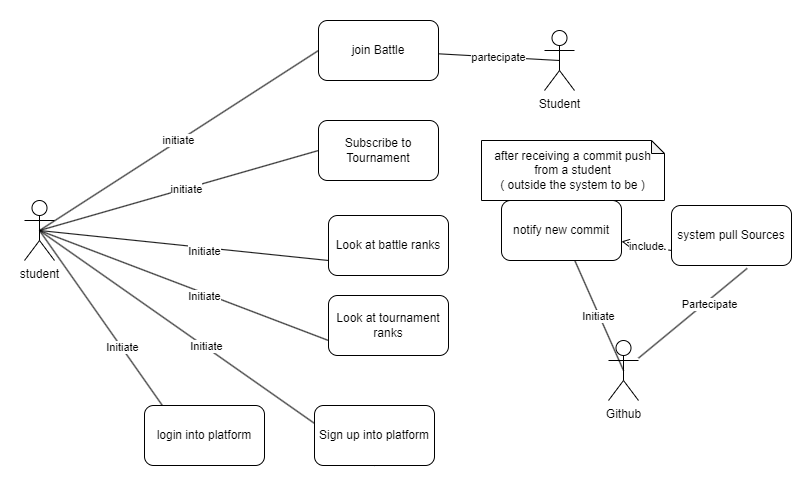
\includegraphics[width=1\linewidth]{misc//Images//UC/StudentScenarios.png}
    \caption{Student Use Case Diagram}
    \label{fig:enter-label}
\end{figure}


\subsubsection{Educator Use Case Diagram}
\begin{figure}[H]
    \centering
    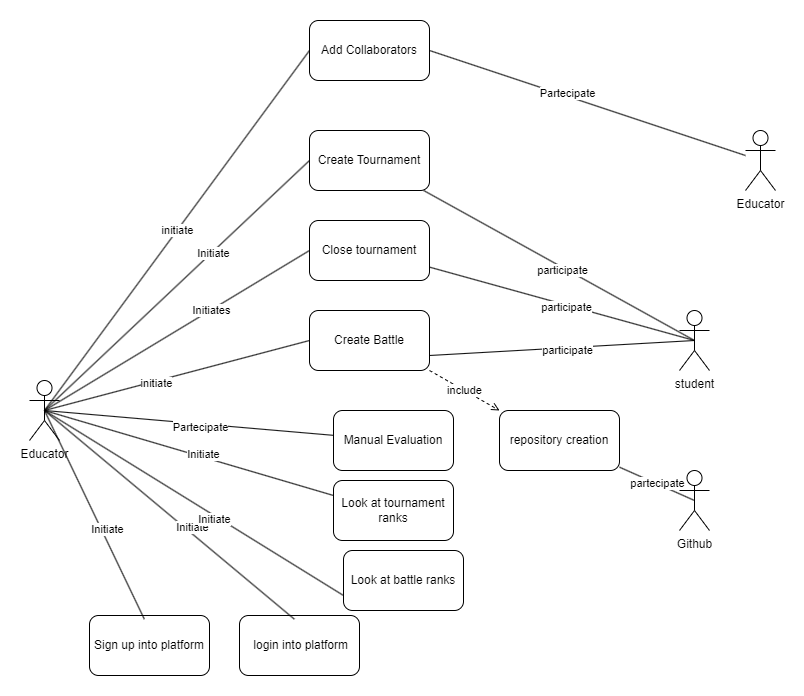
\includegraphics[width=1\linewidth]{misc//Images//UC/EducatorScenarios.png}
    \caption{Educator Use Case Diagram}
    \label{fig:enter-label}
\end{figure}

\subsection{Use Cases}
In this section we analyze the various use cases of the system by describing the actors, entry conditions, event flow, exit conditions and exceptions for all of them.

\newpage
\subsubsection{UC1: Sign Into Platform}
\begin{center}
    \begin{longtable}{lp{0.75\linewidth}}
        \hline
            Actor & Users(Educators, Students)\\
        \hline
            Entry condition & A user accesses the platform for the very first time\\
        \hline
            Event Flow & 1. User reaches the platform\\
                &2. User clicks on "sign in" button\\
                &3. User fills out own info and decides if they want to be an Educator or student\\
                &4. User concludes the registration by clicking "finish" button\\
        \hline
            Exit & User is successfully registered on the platform as either educator or student\\
        \hline
            Exception & Missing or wrong input by user during registration form\\
        \hline
    \end{longtable}
\end{center}


\begin{figure}[H]
    \centering
    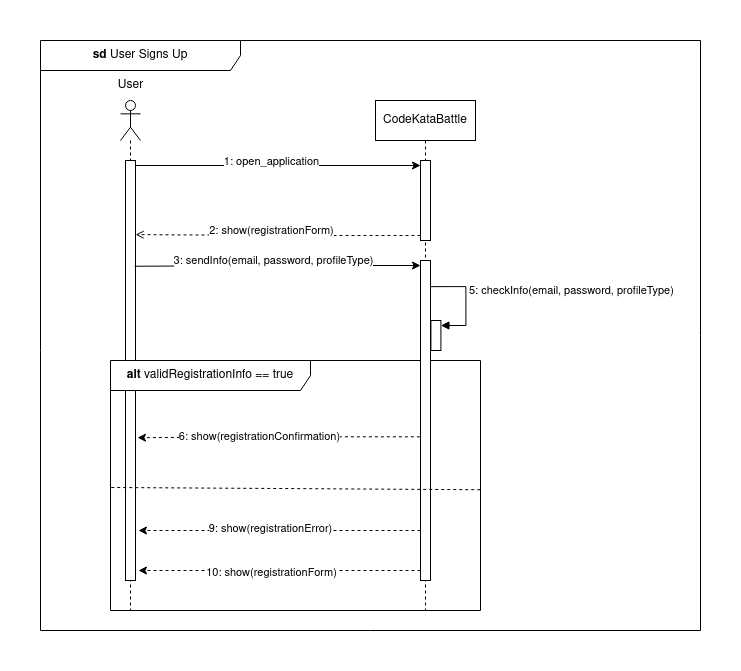
\includegraphics[width=1\linewidth]{misc//Images//UC Diagrams/UC1.png}
    \caption{User Signs Up sequence diagram}
    \label{fig:enter-label}
\end{figure}

\subsubsection{UC2: Log Into Platform}
\begin{center}
    \begin{longtable}{lp{0.75\linewidth}}
        \hline
            Actor & User\\
        \hline
            Entry condition & User is signed into platform\\
        \hline
            Event Flow & 1. User reaches the platform\\
                       & 2. User clicks on "log in" button\\
                       & 3. User fills out email and password used during registration\\
                       & 4. User completes login by clicking "confirm" button\\
        \hline
            Exit & User is successfully logged into platform\\
        \hline
            Exception & Missing or wrong input by user during log in form\\
        \hline
    \end{longtable}
\end{center}

\begin{figure}[H]
    \centering
    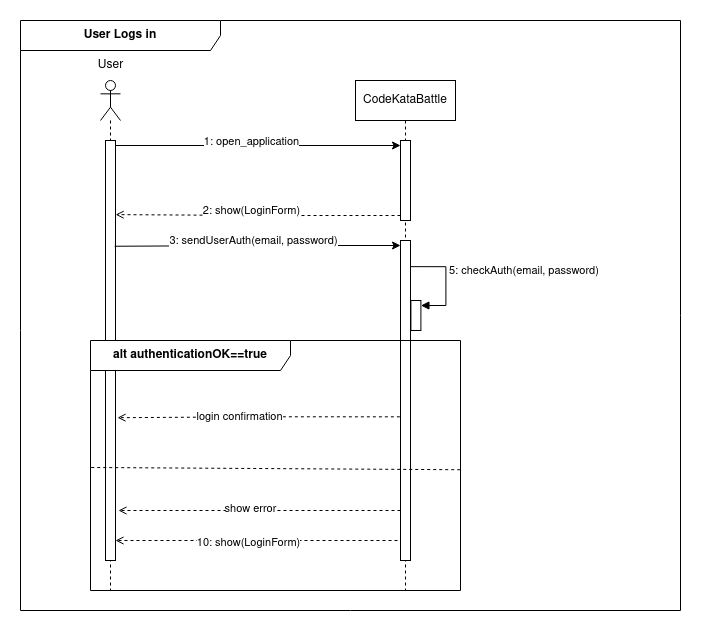
\includegraphics[width=1\linewidth]{misc//Images//UC Diagrams/UC2.png}
    \caption{Create tournament sequence diagram}
    \label{fig:enter-label}
\end{figure}

\newpage
\subsubsection{UC3: Create Tournament}
\begin{center}
    \begin{longtable}{lp{0.75\linewidth}}
        \hline
            Actor & Educator, Students\\
        \hline
            Entry condition & Educator is logged into the platform\\
        \hline
            Event Flow &  1. Educator presses "Create Tournament" button\\
                       &  2. Educator fills out details of tournament\\
                       &  3. Educator adds other collaborators to tournament(other Educators)\\
                       &  4. Educator completes tournament creation\\
                       &  5. Platform notifies all Students of new tournament\\
        \hline
            Exit & Tournament is created successfully \\
        \hline
            Exception & Missing or wrong input by Educator during tournament creation form\\
        \hline
    \end{longtable}
\end{center}

\begin{figure}[H]
    \centering
    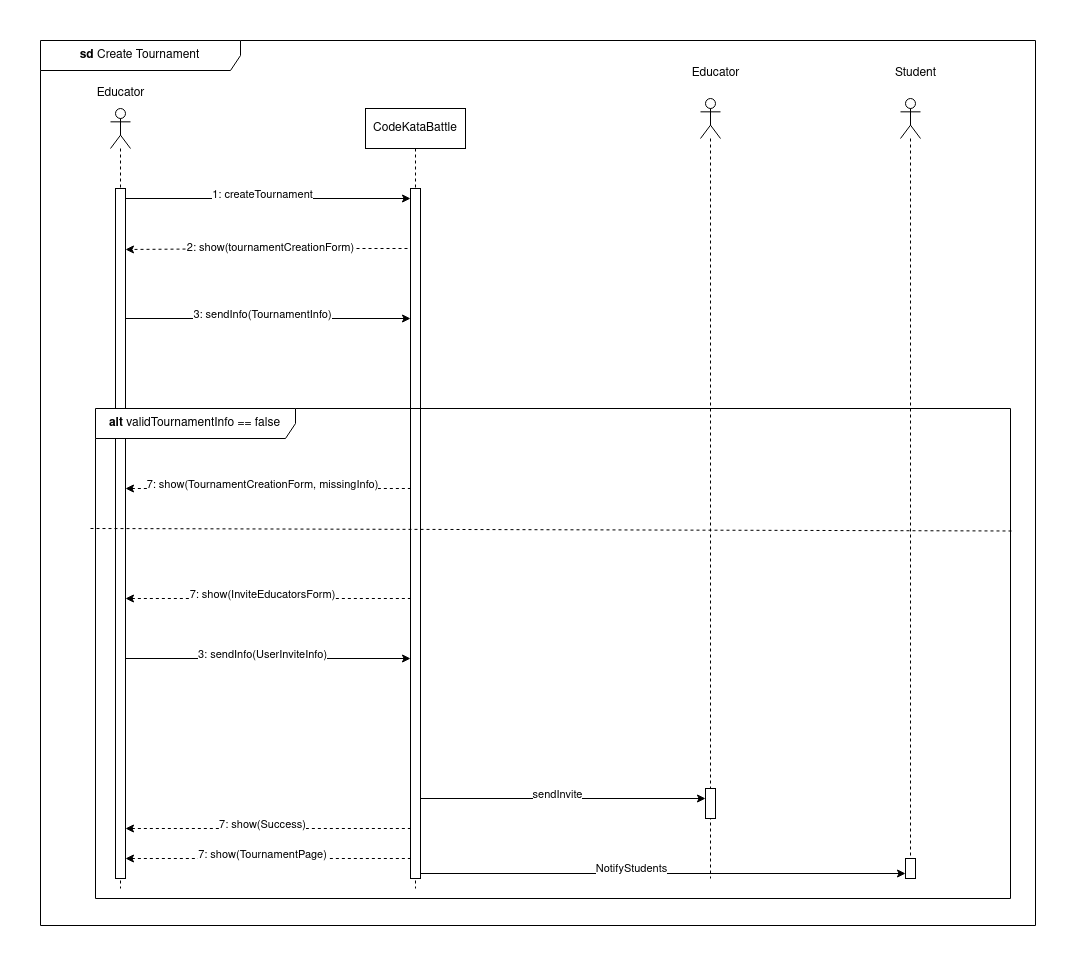
\includegraphics[width=1\linewidth]{misc//Images//UC Diagrams/UC3.png}
    \caption{Create tournament sequence diagram}
    \label{fig:enter-label}
\end{figure}

\newpage
\subsubsection{UC4: Subscribe to Tournament}
\begin{center}
    \begin{longtable}{lp{0.75\linewidth}}
        \hline
            Actor & Students\\
        \hline
            Entry condition & Student is logged into the platform\\
        \hline
            Event Flow & 1. Student is notified of new tournament\\
                       & 2. Student presses "Join tournament" button\\
        \hline
            Exit & Student is subscribed to tournament\\
        \hline
            Exception & \\
        \hline
    \end{longtable}
\end{center}

\begin{figure}[H]
    \centering
    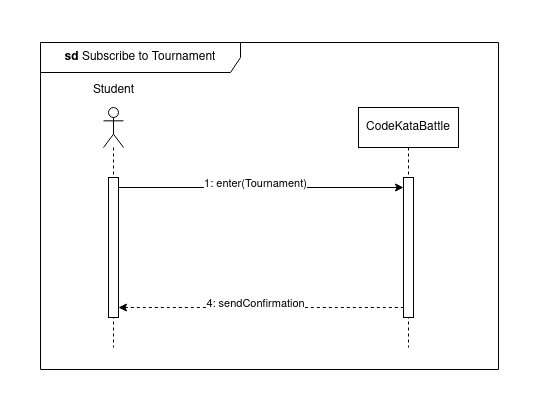
\includegraphics[width=1\linewidth]{misc//Images//UC Diagrams/UC4.png}
    \caption{Subscribe to Tournament sequence diagram}
    \label{fig:enter-label}
\end{figure}

\newpage
\subsubsection{UC5: Create Battle}
\begin{center}
    \begin{longtable}{lp{0.75\linewidth}}
        \hline
            Actor & Educator, Student\\
        \hline
            Entry condition & Educator has logged in and is inside the context of a tournament\\
        \hline
            Event Flow & 1. Educator press "create new battle" button\\
                       & 2. Educator upload the \ac{CK} assignment, tests and project build\\
                       & 3. Educator sets subscription and submission deadlines and group size rules\\
                       & 4. Educator complete battle creation\\
                       & 5. The platform sends notification to all the students subscribed to the tournament\\
        \hline
            Exit & Battle created correctly\\
        \hline
            Exception & Missing or wrong input by Educator\\
        \hline
    \end{longtable}
\end{center}

\begin{figure}[H]
    \centering
    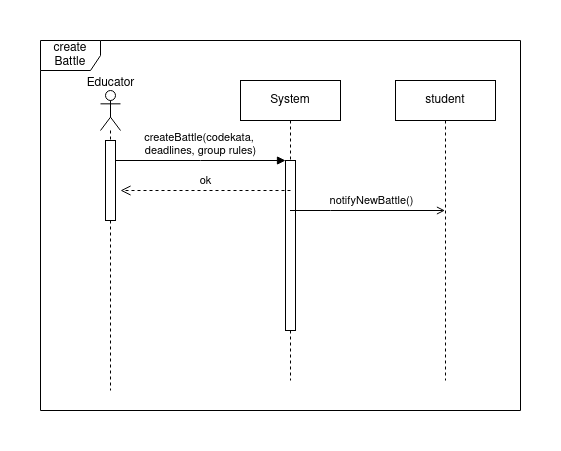
\includegraphics[width=1\linewidth]{misc//Images//UC Diagrams/UC5.png}
    \caption{Create Battle sequence diagram}
    \label{fig:enter-label}
\end{figure}

\newpage
\subsubsection{UC6: Join Battle}
\begin{center}
    \begin{longtable}{lp{0.75\linewidth}}
        \hline
            Actor & Student\\
        \hline
            Entry condition & Student subscribed to a tournament, student logged in, battle available for subscription in tournament\\
        \hline
            Event Flow  & 1. Student press "join battle" button in tournament context\\
                        & 2. platform shows group size rules\\
                        & 3. student uses "invite" button\\
                        & 4. Student inserts other students identifiers\\
                        & 5. other students accepts invite\\
                        & 6. Group of student is created\\
                        & 7. Group of students joins battle\\
        \hline
            Exit & Student group joins battle\\
        \hline
            Exception & \\
        \hline
    \end{longtable}
\end{center}

\begin{figure}[H]
    \centering
    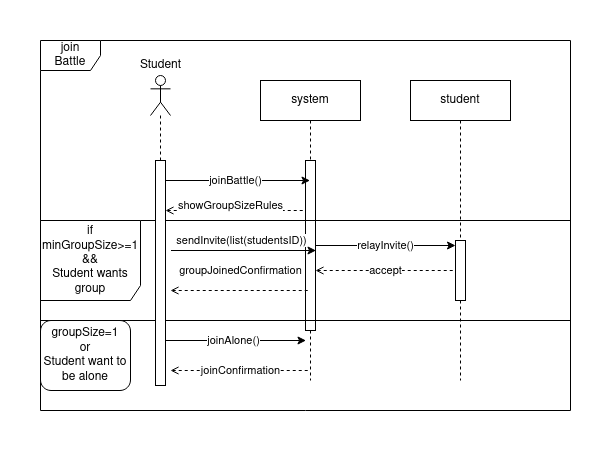
\includegraphics[width=1\linewidth]{misc//Images//UC Diagrams/UC6.png}
    \caption{Join Battle sequence diagram}
    \label{fig:enter-label}
\end{figure}

\newpage
\subsubsection{UC7: Create Repository}
\begin{center}
    \begin{longtable}{lp{0.75\linewidth}}
        \hline
            Actor & Github, Student\\
        \hline
            Entry condition & Subscription deadline of battle expired\\
        \hline
            Event Flow & 1. The platform creates a repository for the codekata battle in github\\
                       & 2. The platform sends to all students subscribed to the battle the link to the repository\\
        \hline
            Exit & Student recieve repository link\\
        \hline
            Exception & \\
        \hline
    \end{longtable}
\end{center}

\begin{figure}[H]
    \centering
    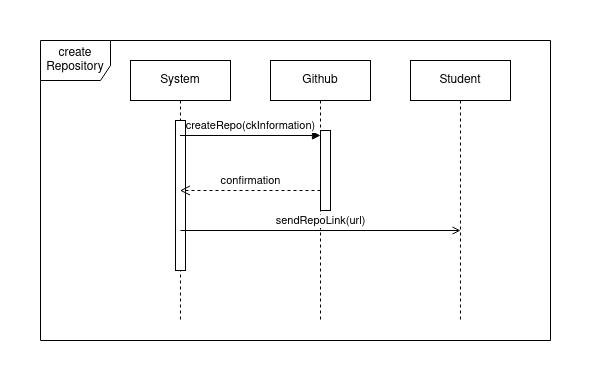
\includegraphics[width=1\linewidth]{misc//Images//UC Diagrams/UC7.png}
    \caption{Create Repository sequence diagram}
    \label{fig:enter-label}
\end{figure}

\newpage
\subsubsection{UC8: Score Commit}
\begin{center}
    \begin{longtable}{lp{0.75\linewidth}}
        \hline
            Actor & GitHub\\
        \hline
            Entry condition & Github notified platform of student commit\\
        \hline
            Event Flow & 1. Platform receives notification of commit\\
                       & 2. Platform pulls sources and compiles them\\
                       & 3. Platform starts evaluation(functional, timeliness, quality)\\
                       & 4. Platform updates score for battle\\
        \hline
            Exit & Battle leader board is updated\\
        \hline
            Exception & Compilation of sources fails\\
        \hline
    \end{longtable}
\end{center}

\begin{figure}[H]
    \centering
    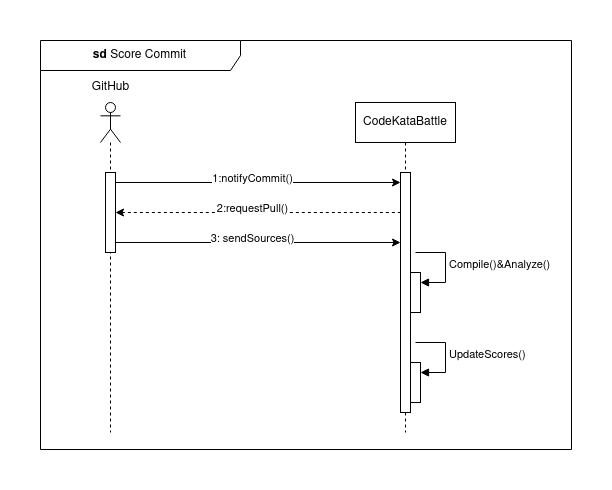
\includegraphics[width=1\linewidth]{misc//Images//UC Diagrams/UC8.png}
    \caption{Score Commit sequence diagram}
    \label{fig:enter-label}
\end{figure}

\newpage
\subsubsection{UC9: View Battle Ranking}
\begin{center}
    \begin{longtable}{lp{0.75\linewidth}}
        \hline
            Actor & User(Educators, Students)\\
        \hline
            Entry condition & Educator is involved with tournament of the battle, student has joined battle\\
        \hline
            Event Flow & 1. User press "view ranking" button in battle context\\
                       & 2.platform shows ranking table\\
        \hline
            Exit & User sees ranking table\\
        \hline
            Exception & \\
        \hline
    \end{longtable}
\end{center}

\begin{figure}[H]
    \centering
    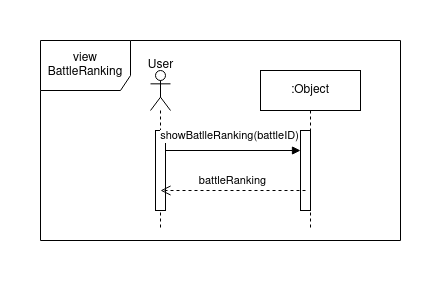
\includegraphics[width=1\linewidth]{misc//Images//UC Diagrams/UC9.png}
    \caption{View Battle Ranking sequence diagram}
    \label{fig:enter-label}
\end{figure}

\newpage
\subsubsection{UC10: Manual Evaluation}
\begin{center}
    \begin{longtable}{lp{0.75\linewidth}}
        \hline
            Actor & Educators\\
        \hline
            Entry condition & Battle deadline Expires\\
        \hline
            Event Flow & 1. Platform notifies educators that battle ha ended and manual evaluation is required(as decided during battle creation)\\
                       & 2. Educators use platform to analyze sources\\
        \hline
            Exit & Educator add a manual score\\
        \hline
            Exception & Educator adds illegal score\\
        \hline
    \end{longtable}
\end{center}

\begin{figure}[H]
    \centering
    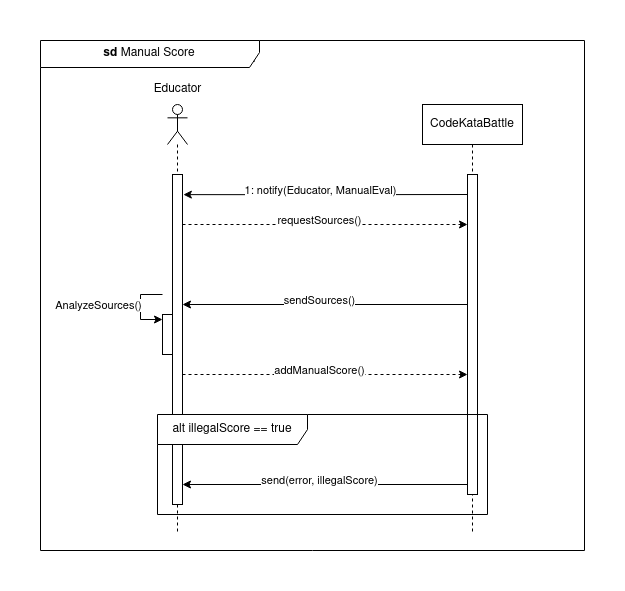
\includegraphics[width=1\linewidth]{misc//Images//UC Diagrams/UC10.png}
    \caption{Manual Evaluation sequence diagram}
    \label{fig:enter-label}
\end{figure}

\newpage
\subsubsection{UC11: Look at tournament ranks}
\begin{center}
    \begin{longtable}{lp{0.75\linewidth}}
        \hline
            Actor & Students, Educators\\
        \hline
            Entry condition & Student or Educator are on the main tournament page and are involved\\
        \hline
            Event Flow & 	Student or educator click on tournament leader-board\\
        \hline
            Exit & 	Platform shows Tournament leader board\\
        \hline
            Exception & Tournament hasn't yet started \\
        \hline
    \end{longtable}
\end{center}

\begin{figure}[H]
    \centering
    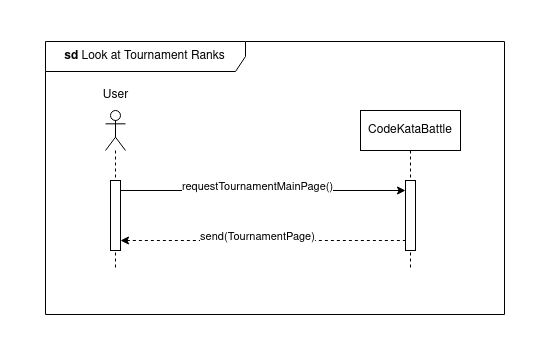
\includegraphics[width=1\linewidth]{misc//Images//UC Diagrams/UC11.png}
    \caption{Look at tournament ranks sequence diagram}
    \label{fig:enter-label}
\end{figure}

\newpage
\subsubsection{UC12: Close Tournament}
\begin{center}
    \begin{longtable}{lp{0.75\linewidth}}
        \hline
            Actor & Educator, Student\\
        \hline
            Entry condition & Educator logged in, Tournament still ongoing, no ongoing battle\\
        \hline
            Event Flow & 1. Edu press "close tournament" in the tournament context\\
& 2. The platform closes the tournament\\
& 3. The platform notifies all the students subscribed to the tournament\\
        \hline
            Exit & Tournament closed, platform notifies students\\
        \hline
            Exception & \\
        \hline
    \end{longtable}
\end{center}

\begin{figure}[H]
    \centering
    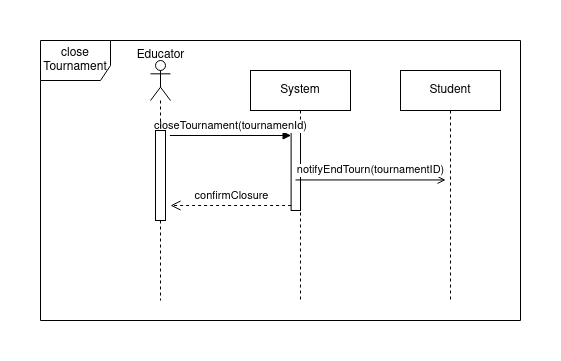
\includegraphics[width=1\linewidth]{misc//Images//UC Diagrams/UC12.png}
    \caption{Close Tournament sequence diagram}
    \label{fig:enter-label}
\end{figure}


\newpage
\subsection{Mapping on requirements}

\begin{center}
    \begin{longtable}{l p{0.75\linewidth}}
        \hline
            \textbf{Use Case} & \textbf{Requirements}\\
        \hline
            UC1 & R10\\
        \hline
            UC2 & R5, R6\\
        \hline
            UC3 & R6, R2.1, R1, R14\\
        \hline
            UC4 & R5, R3\\
        \hline
            UC5 & R6, R2, R2.1, R2.2, R2.3, R2.4, R2.5, R15\\
        \hline
            UC6 & R5, R4, R4.1, R15\\
        \hline
            UC7 & R18, R19\\
        \hline
            UC8 & R9, R9.1, R13, R13.1\\
        \hline
            UC9 & R5, R6, R13, R13.1\\
        \hline
            UC10 & R6, R7, R2.5, R16\\
        \hline
            UC11 & R5, R6, R8, R8.1\\
        \hline
            UC12 & R6, R17, R11\\
        \hline
        
    \end{longtable}
\end{center}

\section{Design Constraints}
\subsection{Standards compliance}
First of all, the system should respect all the laws regarding privacy and data treatment and exchange with third parties (i.e. CPOs); to work in Europe, the system should respect the EU GDPR. In particular, a general description of the main principles that data should have in order to guarantee their privacy is given in Art. 5 of the GDPR document.

\subsection{Hardware limitations}
There are no hardware contraints.

\subsection{Any other constraint}
There are no other constraints.

\section{Software System Attributes}
\subsection{Reliability}
The system should be able to restart automaticly shortly after an interruption and recover the previous backupped state.

\subsection{Availability}
The system should be operative at least 99\% of the time to avoid the impairment of activities with deadlines and in case of downtime the system should recover any missed notification received from GitHub on group commit in battles when it restarts.

\subsection{Security}
The system should ensure safety of the user credentials and it should keep log of access and of sensible operations, such as in the case of educator closing a tournament or manually evaluation of sources, to avoid malicious use of the educator authority.

\subsection{Maintainability}
The development should follow good practice for maintainability, such as dividing the system in enough modules depending on the functionalities. This is necessary in order to facilitate maintenance and substitution of modules. Every functionality needs to be well documented.

\subsection{Portability}
The platform as a website should behave as expected on at least the most used browsers, without requiring additional effort from the end user. The back end should be written in a language that ensures portability and its functionalities should not be reliant on a particular compiler of system.
